\section{Problem Domain}
\label{sec:domain}
%A thorough understanding of the problem domain is not only crucial to the
%development of a decent DSL, but also for its understanding.

This section describes the problem domain underlying AiryScript. It does not
contain the elements that were already present in the original commissioning
made by GlobAir Inc..

Subsection \ref{sec:domain_description} documents elements that are
missing from the original domain description.
%
Subsection \ref{sec:domain_analysis} contains an analysis of the entire problem
domain. It lists all the relations that exist in between domain elements.
It thereby acts as an important basis for the design of AiryScript.

\subsection{Domain description}
\label{sec:domain_description}
This subsection documents all the additional elements that are missing from the
original job description made by GlobAir Inc.. It elaborates and justifies all
elements that do not have domain expert David Clarke as their source.


\subsubsection{Unsupported operations}
\label{sec:unsupported}
This subsection gives an overview of some of the more important operations that
are currently not supported by AiryScript.

There is some functionality that might be required of AiryScript before it goes
live. AiryScript does currently not provide this functionality because it is
still just a proof of concept, and the assignment does not mention it.
\begin{itemize}
  \item Booking flights.
  \item Retrieving information from the database.
  \item Keeping track of individual airplanes.
\end{itemize}

Also, in consultation with the domain expert, AiryScript does currently not
provide the following functionality.
\begin{itemize}
  \item Overbooking, i.e. the number of seats in an airplane has to be equal to
    the number of seats the user has to specify prices for.
  \item Codeshare agreements, i.e. a flight has to map onto a single airline
    company.
\end{itemize}

\subsubsection{Unspecified, supported operations}
\label{sec:unspecified_supported}
In consultation with the domain expert, AiryScript provides the following
functionality that is not specified in the original assignment.
\begin{itemize}
  \item Changing the airplane type of flight templates. In addition, AiryScript
    changing the airplane type of specific flights.
    It does not currently support specifying changes of airplane type over time.    %By changing the airplane
    %type of flight templates, the history track of flown flights is not changed,
    %and neither are any of the specific instances of the flight templates for
    %which another airplane was already specified.

    %AiryScript also supports changing the airplane type of specific flights.
\end{itemize}


\subsubsection{Additional decisions}
\label{sec:additional_decisions}
When implementing AiryScript, we also made some decisions that we did not
discuss with the domain expert.
\begin{itemize}

  \item The original domain description is not specific on how elaborate
    descriptions of new flights can be. The assignment describes flight
    templates that correspond to weekly recurring flights. The assignment also
    hints that there can also be individual, non-recurring flights and that the
    number of flights.
    
    AiryScript supports defining single flights and weekly flight patterns,
    possibly with multiple flying days per week and multiple flights per day. It
    also supports specifying multiple, possibly disconnected time periods over
    which the flight pattern is valid.
    
    This means that users can make statements like the following.
    \begin{quote}
      There is a flight every Monday at 13:00 and Friday at 17:30 starting from
      August 2013 and ending at September 2013. Starting from October 2013 and
      until the end of times, only the flight on Monday remains.
    \end{quote}
    This also means that users cannot specify a flight pattern occurring every
    third Friday of the month.
    
    AiryScript supports manually adding flights to flight codes. In this
    way, exceptional one-time only flights do not require modifying the flight
    that corresponds to the flight code. Also, users who really want to
    schedule flights each third Friday of the month can use this functionality
    to manually add flights.

  \item AiryScript supports changing the prices of individual seats of
    individual flights and the prices of flight templates, possibly only over a
    specified period. Users can also use seat types to specify groups of seats
    for which to change the price; these seat types are specified by the type of
    airplane.

    Binding seat types to airplanes has advantages and disadvantages. The
    greatest advantage is that users can use seat types to specify prices on a
    newly created flight, without first having to specify how many seats
    there are for each type of seat. Also, usually different seat types actually
    map to different types of seats, like seats with extra leg space. The
    greatest disadvantage is that it currently makes it impossible to specify
    additional pricing groups that are valid only for a specific flight.

    We feel that the advantages of binding seat types to airplane types outweigh
    its disadvantages. Users can still specify any prices they want, because
    they can change prices of individual seats. If required, it would also
    certainly be possible to provide names for groups of seats that are tied to
    individual flights or flight templates.

    AiryScript does not support changing prices as a function of time.

  \item AiryScript always requires users to specify an airplane type when
    creating individual flights or flight templates.

    We believe this restriction is justified, because AiryScript supports
    changing the airplane type of a flight after its creation. If a user really
    has no idea of the type of airplane that is used for the flight he is
    inserting, he or she can create a dummy airplane.

    When creating a dummy airplane, a user should configure it
    with sensible seating information. Special care should be given to seat
    types, because otherwise changing airplane types could go wrong. The next
    bullet point provides more information.

  \item AiryScript provides support for changing airplane types, but it is very
    basic. Since we keep track of prices of individual seats and not just seat
    types, it is not generally possible to change airplane type without
    requiring some additional information.

    When changing to a smaller airplane, pricing information is inevitably lost.
    AiryScript cannot know which prices the user wants to keep: the highest
    prices, the lowest prices, the highest prices after matching seat types, if
    that is even possible? Even when changing the airplane type to a type that
    has more seats of every type, there are several policies we could use to set
    the price of the surplus seats.  AiryScript could provide syntax that lets
    the user specify the conversion policy it should use, but as AiryScript is,
    at this point, a proof of concept, it does not currently support such
    syntax.

    Instead, AiryScript sets the prices of all seats with seat type $t$ in the
    new airplane type to the same price: the price of the seat in the old
    airplane with seat type $t$ that has the lowest seat number. If the old
    airplane has no seats of type $t$, it sets the price to the price of least
    expensive seat on the old airplane.

    Note that in the common case in which the new and the old airplane only
    contain seats of common seat types and all seats of the same type have the
    same price, this method works as expected. All seats of type $t$ in the new
    airplane will have the same price as the seats of type $t$ in the old
    airplane.

    We believe our approach here is justified. The rule above covers the only
    case where there is an obvious best price conversion policy. If a user is
    unsatisfied with the default conversion rule, he can always respecify prices
    after conversion. No policy can always save you from this.
\end{itemize}


\subsection{Domain analysis}
\label{sec:domain_analysis}
This subsection analyses the domain elements introduced by the previous two
subsections. It acts as a basis for decisions on the syntax of AiryScript.

We start off with a quick note. One of the more confusing aspects of the domain
description is the description of a flight. When the domain expert refers to a
flight it can mean either an individual flight or a recurring flight. To avoid
confusion this document uses flight only in its first meaning. It uses
\jdef{flight template} or simply \jdef{template} instead of flight in its second
meaning.

\begin{figure}
  \def\svgwidth{\textwidth}
  %\subsection{SQL Database}
  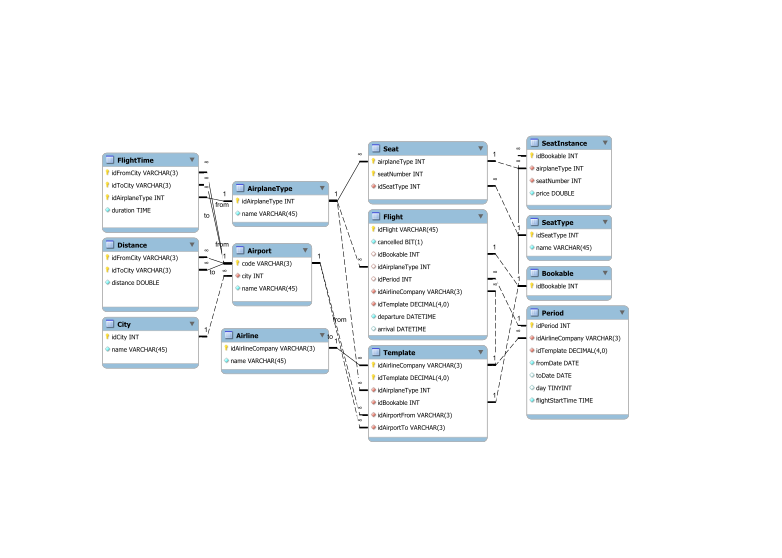
\includegraphics[width=\textwidth]{database}
  \caption{Structure of AiryScript’s underlying relational database. Because our
  database maps very closely to the domain, this figure can also be seen as a
domain model.
Lines in between tables indicate the use of foreign keys. Solid lines indicate
that the foreign key is part of the primary key of one of the tables. All the
other lines are dashed.}
  \label{fig:database}
\end{figure}

Figure \ref{fig:database} forms the base of our discussion of the domain. It
displays the relational database underlying AiryScript, but as it has a very
clean structure and is 3NF-normalized, it can also serve as the domain model of
AiryScript.

\begin{description}
  \item[\dbf{City}] instances correspond to a city, e.g. the City of New York. A
    city has a name and is bound to several airports.

    Since there can be multiple cities with the same name (e.g. 13 cities, 11
    towns and 14 townships in the USA are called Springfield), we do not use
    \dbf{name} as the identifier of city.

  \item[\dbf{Airport}] instances correspond to an airport. Airports are identified by a
    three-character code, have a name and are situated in a city. AiryScript
    records flight times and distances between some pairs of airports. 
    
    Note that there can be multiple airports in the same city, to cover cases
    like the Newark and JFK airports in the City of New York.

  \item[\dbf{Distance}] corresponds to the distance in between two airports.
    Note AiryScript does not assume the distance from airport $a$ to airport $b$
    to be equal to the distance from airport $b$ to airport $a$.

    There does not necessarily have to be a \dbf{Distance} entry for every pair
    of airports in \dbf{Airport}, but there has to be such an entry for all
    pairs of airports for which there are flights. This is enforced when users
    try to define new templates or change templates (also see \dbf{Template}).

  \item[\dbf{FlightTime}] instances correspond to the flight time in between to airports
    for a specific type of aircraft.
    
    We do not merge distance and flight time because this violates 2NF
    normalization: unlike flight time, distance is not dependent on the type of
    aircraft.

    There does not necessarily have to be a \dbf{FlightTime} entry for all
    combinations of types of airplanes and pairs of airports, but there has to
    be an entry for all such combinations for which there are flights. This is
    enforced when users try to define new templates or change templats (also see
    \dbf{Template}).

  \item[\dbf{AirplaneType}] instances correspond to a specific type of airplane, e.g.
    Boeing 727. An airplane type consists of a name and is bound to several
    seats. We say that an airplane type $t$ ‘has’ $n$ seats if there are $n$
    instances of \dbf{Seat} linked to $t$.

    Note that AiryScript does not keep track of individual airplanes.

  \item[\dbf{Seat}] instances correspond to a specific seat on a type of airplane. Note
    that \dbf{Seat} does \emph{not} correspond to a single seat, as there can be
    multiple airplanes of the same type. The only property of a seat is its seat
    type.

    Each seat is bound to a instances of \dbf{SeatInstance} for every flight or
    template. Instance of \dbf{SeatInstance} can correspond to actual physical
    seats.

  \item[\dbf{SeatType}] instances correspond to a type of seat. Examples of seat
    types include business, first class and economic seats. The user is free to
    make as much seat types as he or she wants.

    Seat types consist of disjoint groups of seats and are linked to airplane
    types. We advise users to set seat types so that seats with different seat
    types correspond to different types of seat in the real world and vice
    versa.
    
    Seat types group seats, and AiryScript uses these groups to set prices and
    to convert prices when the user changes the airplane type of flights, as
    described in section \ref{sec:additional_decisions}.

  \item[\dbf{AirlineCompany}] instances correspond to airline companies. Airline
    companies are identified by a three-character code and have a name.

    Each airline company can be linked to several flight templates. Those flight
    templates are in turn linked to flights. In this way, airline companies are
    linked to flights.

  \item[\dbf{Template}] instances describe a flight template, the most
    complicated domain element modeled by AiryScript. A flight template is
    identified by a FLN (FLight Number), which consists of the airline code
    followed by three or four digits.
    
    \begin{itemize}
      \item Templates specify an origin and destination city.  AiryScript
        refuses to add templates with or change templates to couples of cities
        and airplane types for which there are no \dbf{Distance} and
        \dbf{FlightTime} instances.  Because of this, \dbf{Template} instances
        are guaranteed to have access to distance and flight time information.
      \item Templates specify an airplane type.
      \item A template describes when flights occur through \dbf{Period}
        instances. More information is in the description of \dbf{Period}.
      \item Each template has as much seat instances as there are seats in its
        airplane type.
    \end{itemize}

    Whenever necessary, AiryScript automatically instantiates flights from a
    flight template. This process is transparent to the user, so that for all
    the user cares, specifying a template that recurs every Wednesday from now
    until the end of times actually creates an infinite number of \dbf{Flight}
    instances. AiryScript uses the seat instances and airplane type of the
    template as default values for the underlying flights; of course, these
    default values can always be changed. The description of \dbf{Flight}
    provides more information on the link between a template and its underlying
    flight instances.

  \item[\dbf{Flight}] instances describe a flight. All flights are linked to a
    flight template, and therefore ‘inherit’ all the properties of a template. A
    flight differs from a template by specifying an actual time (\dbf{from})
    instead of describing periods over which it is valid as is the case for
    templates.
   % When a \dbf{Flight} instance is actually created remains transparent for the
   % users of AiryScript. Even if \dbf{Flight} instances are created, they remain
   % very tightly linked to their underlying templates until some of their
   % properties are changed.

    Templates define airplane type, pricing and travel time, which are
    used as the default values for flights underlying the template. Until a user
    changes the pricing or travel time of a specific flight, airplane type,
    pricing and travel time of the flight changes together with changes to its
    template.
    
    As an example, suppose we have a template $t$ that describes a flight every
    Friday and a flight $f$ that is the instance of $t$ next Friday. As long as
    the user did not change the price of any seat in $f$, changing the price of
    seat $s$ in $t$ changes the price of seat $s$ in $f$ as well. As soon as the
    user specifies the price of any seat (not necessarily $s$) in $f$
    specifically, AiryScript breaks the pricing information link and airplane
    type link between $f$ and $t$. Changing the price of $s$ in $t$ or the
    airplane type in $t$ then no longer has any influence on the price of $s$ in
    $f$. AiryScript unlinks airplane types together with pricing information
    because pricing information is not generally compatible with different
    airplane types.
    
    The example is also valid for the arrival time of $f$: as long as the user
    does not specify an explicit arrival time \dbf{to} for $f$, AiryScript
    assumes it to be equal to $f$’s departure time \dbf{from} plus the travel
    time of $f$ specified through $t$. Changing the travel time in $t$ therefore
    changes the arrival time of $f$. As soon as we change the arrival time in
    $f$ specifically, for example because $f$ is delayed, AiryScript breaks this
    connection to $t$.
    
    The properties of \dbf{Flight} instances that lie in the past never change
    together with changes to their templates.

    If a flight was automatically created from a template, it also carries a
    link to the period it was created from. If a user removes the period from
    the template, AiryScript removes all flights that were automatically created
    from the period.

  \item[\dbf{Period}] instances define days on which there are flights and are
    linked to a specific template. The template is valid over the union of all
    period instances it is linked to.

    A period instance $p$ has two mandatory properties: the hour when flights
    defined by that period takes off and a starting time. When not specifying
    any of its other properties, a period defines a flight that takes off every
    day at the specified hour starting from the starting time until the end of
    times.

    Optionally, users can attach an end time in addition to a start time. In
    this way he or she defines a time period, for example the time period in
    between 11/1/2013 and 11/2/2013. $p$ is then only valid over that time
    period. When not specifying any other properties besides the hour, $p$
    specifies a flight that takes off every day during the time period, for
    example every day between 11/1/2013 and 11/2/2013 (inclusive).

    Optionally, we can also attach a day to $p$. $p$ is then not valid every
    day of the week, but only during the specified day.

    As an example, take the period with properties \dbf{fromDate} = 11/1/2013,
    \dbf{toDate} = 11/2/2013, \dbf{day} = monday and \dbf{flightStartTime} =
    12:00. Such a period defines a flight at 12:00, every monday in the period
    in between 11/1/2013 and 11/2/2013.

    Adding a period to a template generally creates new flights. Deleting a
    period from a template deletes all flights from the template that were
    spawned from that period.
    
  \item[\dbf{Bookable}] is sort of a superclass for \dbf{Flight} and
    \dbf{Template}. It is the only element in the database that really does not
    match a domain element.

  \item[\dbf{SeatInstance}] instances are identified by a flight or a template
    and a seat of the airplane type of that flight or template. The only
    property of a seat instance is its price, but in the future AiryScript could
    use seat instances to store booking information.
    
    Seat instances correspond to instances of seats for specific flights or
    templates. The seat instances that are linked to flights actually correspond
    to physical seats on some physical airplane. The seat instances that are
    linked to templates serve as ‘default seats’ for flight instances of that
    template.
\end{description}
